\documentclass{beamer}
\usetheme{Pittsburgh} 
%\documentclass{scrartcl}

\usepackage[utf8]{inputenc}
\usepackage{default}
\usepackage[procnames]{listings}
\usepackage{graphicx}
%\usepackage[toc,page]{appendix}
\usepackage{caption}
\usepackage{hyperref}
\usepackage{color}
%\usepackage{csvsimple}
\usepackage{float}
\usepackage[T1]{fontenc}


%Bibliogrpahy?
%\usepackage{bibentry}
%\nobibliography*
%\bibentry{ }

%Python
\definecolor{keywords}{RGB}{255,0,90}
\definecolor{comments}{RGB}{0,0,113}
\definecolor{red}{RGB}{160,0,0}
\definecolor{green}{RGB}{0,150,0}
\lstset{language=Python,
    basicstyle=\ttfamily\scriptsize,
    keywordstyle=\color{keywords},
    commentstyle=\color{comments},
    stringstyle=\color{red},
    identifierstyle=\color{green},
    breaklines = true,
    columns=fullflexible,
    %Numbering and tabs
    %numbers=left,
    %numberstyle=\tiny\color{gray},
    %stepnumber=2,
    %numbersep=1em,
    tabsize=4,
    showspaces=false,
    showstringspaces=false}


\begin{document}

\title{Learning and Adaptivity}
\subtitle{Predicting energy consumption of heat pumps.}
\author{
  \href{daiem.ali@smail.inf.h-brs.de}{Ali, Daiem}: \href{https://github.com/daiemna}{github.com/daiemna}\\
  \href{christophe.quignon@smail.inf.h-brs.de}{Quignon, Christophe}: \href{https://github.com/ChrisQuignon}{github.com/ChrisQuignon}
  %Familyname, Name
} 
\institute{Hochschule Bonn Rhein Sieg}
\date{\today}

\begin{frame}
\titlepage{}
\end{frame}
	

\begin{frame}
\frametitle{Data}

%what is the problem what is the data wheat is the purpose

\end{frame}


\begin{frame}
\frametitle{Analysis}

%correlation
%seasonal decomposition
\begin{figure}[H]
  %\raggedleft
  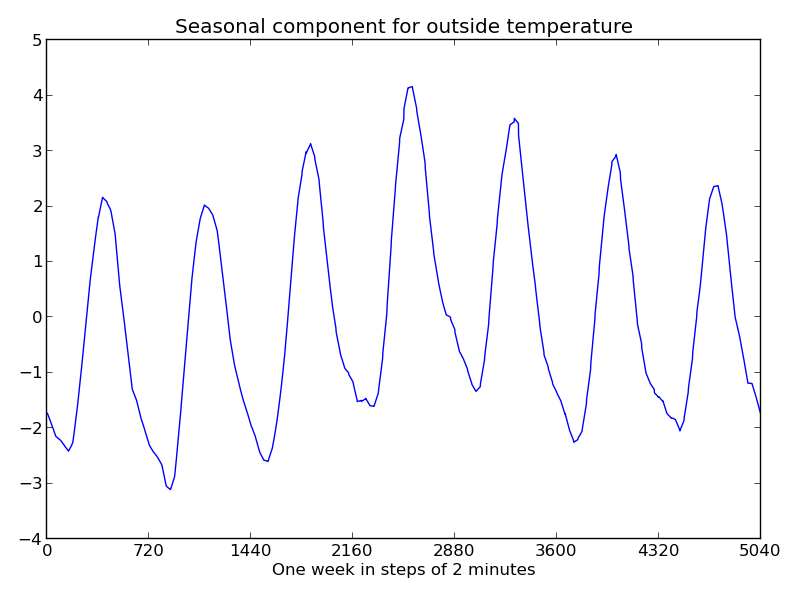
\includegraphics[width=0.6\linewidth]{img/season-outside_temperature.png}
  \caption{Correlation of the datasets.}
  \label{fig:correlation}
\end{figure}

%Exclusion of precipitation`
\begin{figure}[H]
  %\raggedleft
  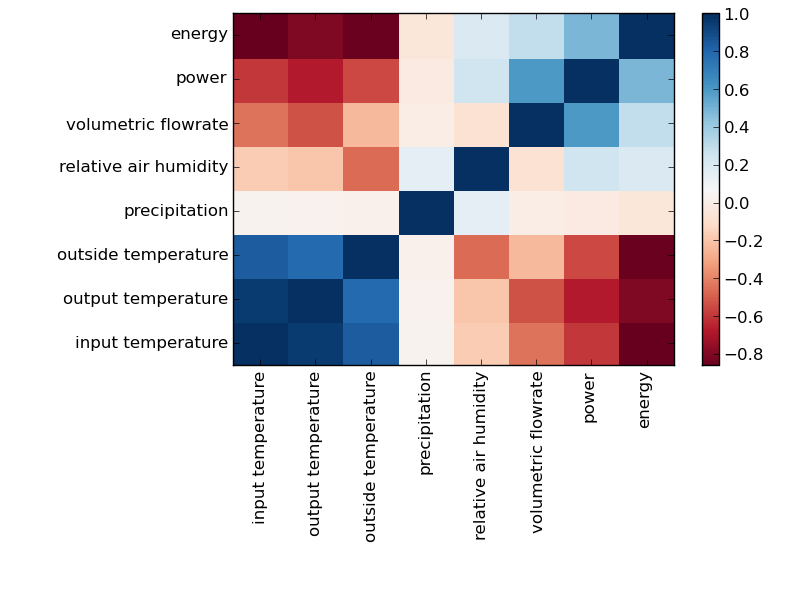
\includegraphics[width=0.6\linewidth]{img/correlation.png}
  \caption{Correlation of the datasets.}
  \label{fig:correlation}
\end{figure}

\end{frame}

\begin{frame}
\frametitle{Methods}

%sliding window
\begin{figure}[H]
  %\raggedleft
  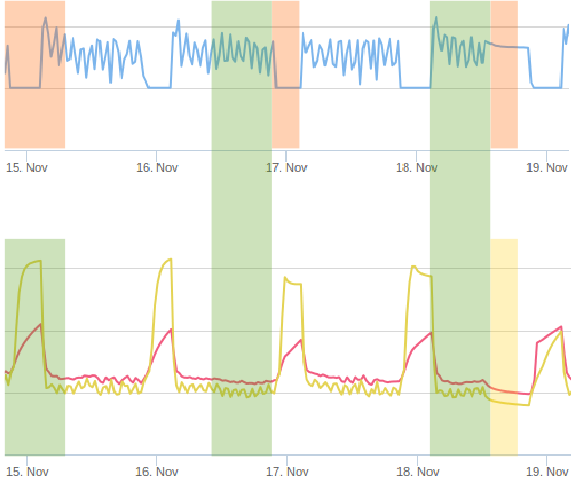
\includegraphics[width=0.6\linewidth]{img/regpred.png}
  \caption{Correlation of the datasets.}
  \label{fig:correlation}
\end{figure}
%gradient boost
%

\end{frame}

\begin{frame}
\frametitle{Conclusion}

\begin{figure}[H]
  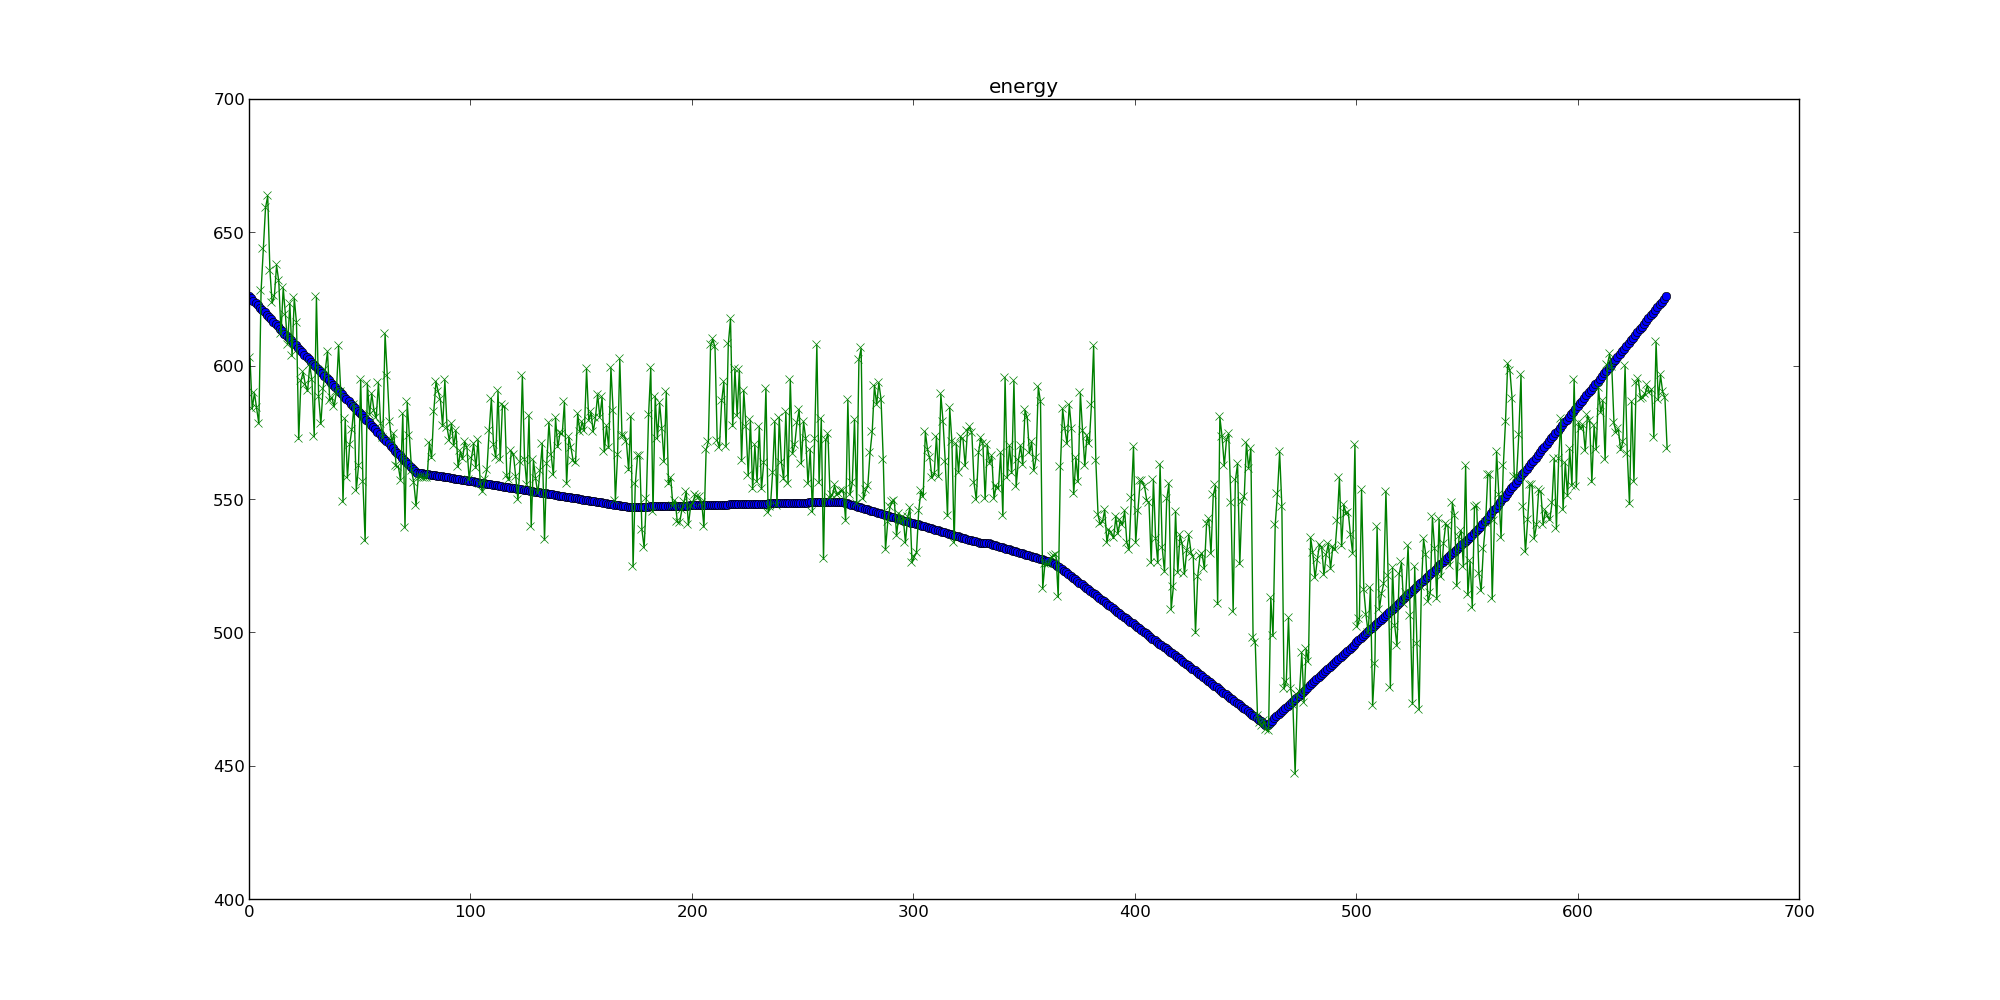
\includegraphics[width=0.6\linewidth]{img/predict-energy-53--0p520.png}
  \caption{Prediction of the energy using the sliding window approach.}
  \label{fig:Prediction}
\end{figure}


%best result:
%sliding window with DOY
%Prediction output

%score/error
%application conclusion

\end{frame}



%CONTENTS
%NOTES

%\begin{frame}[fragile, allowframebreaks]
%\frametitle{}
%\framesubtitle{}
%give your initials so we know whom to bug
%tabulars and long boring stuff is in \scriptsize

%\end{frame}


%COPY AND PASTE FROM HERE

%\begin{enumerate}
% \item 
%\end{enumerate}

%\hyperref{link}{text}

%\begin[Language=Python]{lstlisting}
%#PYTHON CODE HERE
%\end{lstlisting}

%\lstinputlisting[Language=Python]{ }

%\begin{figure}
% \center
% \includegraphics[width= cm]{ }
% \caption{}
%\end{figure}

%BIBLIOGRPAHY?
%\bibliographystyle{ieee}%amsalpha
%\bibliography{ }

\end{document}
